\documentclass[12pt]{article}
\usepackage[margin=2.5cm]{geometry}
\usepackage{enumerate}
\usepackage{amsfonts}
\usepackage{amsmath}
\usepackage{fancyhdr}
\usepackage{amsmath}
\usepackage{amssymb}
\usepackage{amsthm}
\usepackage{mdframed}
\usepackage{graphicx}
\usepackage{subcaption}
\usepackage{adjustbox}
\usepackage{listings}
\usepackage{xcolor}
\usepackage{booktabs}
\usepackage[utf]{kotex}
\usepackage{hyperref}

\definecolor{codegreen}{rgb}{0,0.6,0}
\definecolor{codegray}{rgb}{0.5,0.5,0.5}
\definecolor{codepurple}{rgb}{0.58,0,0.82}
\definecolor{backcolour}{rgb}{0.95,0.95,0.92}

\lstdefinestyle{mystyle}{
    backgroundcolor=\color{backcolour},
    commentstyle=\color{codegreen},
    keywordstyle=\color{magenta},
    numberstyle=\tiny\color{codegray},
    stringstyle=\color{codepurple},
    basicstyle=\ttfamily\footnotesize,
    breakatwhitespace=false,
    breaklines=true,
    captionpos=b,
    keepspaces=true,
    numbers=left,
    numbersep=5pt,
    showspaces=false,
    showstringspaces=false,
    showtabs=false,
    tabsize=1
}

\lstset{style=mystyle}

\pagestyle{fancy}
\renewcommand{\headrulewidth}{0.4pt}
\lhead{CSC 373}
\rhead{Worksheet 5}

\begin{document}
\title{CSC373 Worksheet 5}
\maketitle

\begin{enumerate}[1.]
    \item \textbf{CLRS 26.1-3:} Suppose that a flow network $G = (V,E)$ violates the assumption that the network
    contains a path $s \rightsquigarrow v \rightsquigarrow t$ for all vertices  $v \in V$ . Let $u$ be a vertex for which there
    is no path $s \rightsquigarrow u \rightsquigarrow t$ . Show that there must exist a maximum flow $f$ in $G$ such
    that $f(u,v) = f(v,u) = 0$ for all vertices $v \in V$.

    \item \textbf{CLRS 26.1-6:} Professor Adam has two children who, unfortunately, dislike each other. The problem
    is so severe that not only do they refuse to walk to school together, but in fact
    each one refuses to walk on any block that the other child has stepped on that day.
    The children have no problem with their paths crossing at a corner. Fortunately
    both the professor’s house and the school are on corners, but beyond that he is not
    sure if it is going to be possible to send both of his children to the same school.
    The professor has a map of his town. Show how to formulate the problem of determining
    whether both his children can go to the same school as a maximum-flow
    problem.

    \item \textbf{CLRS 26.1-7:} Suppose that, in addition to edge capacities, a flow network has \textbf{vertex capacities}.
    That is each vertex $v$ has a limit $l(v)$ on how much flow can pass though $v$. Show
    how to transform a flow network $G = (V,E)$ with vertex capacities into an equivalent
    flow network $G' = (V',E')$ without vertex capacities, such that a maximum
    flow in $G'$ has the same value as a maximum flow in $G$. How many vertices and
    edges does $G'$ have?

    \item \textbf{CLRS 26.2-6:} Suppose that each source $s_i$ in a flow network with multiple
    sources and sinks produces exactly $p_i$ units of flow, so that $\sum\limits_{v \in V} f(s_i,v) = p_i$.
    Suppose also that eeach sink $t_j$ consumes exactly $q_j$ units, so that $\sum\limits_{v \in V} f(v, t_j) = q_j$,
    where $\sum\limits_{i} p_i = \sum\limits_{j} q_j$. Show how to convert the problem of finding a flow $f$
    that obeys these additional constraints into the problem of finding a maximum flow in a single source, single-sink
    flow network.

    \item \textbf{CLRS 26.2-9:} Suppose that both $f$ and $f'$ are flows in a network $G$ and we compute flow $f \uparrow f'$.
    Does the augmented flow satisfy the flow conservation property? Does it satisfy the capacity constraint?

    \item \textbf{CLRS 26.2-11:} The \textbf{edge connectivity} of an undirected graph is the minimum number $k$ of edges
    that must be removed to disconnect the graph. For example, the edge connectivity
    of a tree is 1, and the edge connectivity of a cyclic chain of vertices is 2. Show
    how to determine the edge connectivity of an undirected graph $G = (V,E)$ by
    running a maximum-flow algorithm on at most $\lvert V \rvert$ flow networks, each having
    $O(V)$ vertices and $O(E)$ edges.

    \item \textbf{CLRS 26.2-13:} Suppose that you wish to find, among all minimum cuts in a flow network $G$ with
    integral capacities, one that contains the smallest number of edges. Show how to
    modify the capacities of $G$ to create a new flow network $G'$ in which any minimum
    cut in $G'$ is a minimum cut with the smallest number of edges in $G$.

    \item \textbf{CLRS 26-1:} \textbf{Escape problem}

    An $n \times n$ grid is an undirected graph consisting of $n$ rows and $n$ columns of vertices,
    as shown in Figure 26.11. We denote the vertex in the $i^{th}$ row and the $j^{th}$ column
    by $(i, j)$. All vertices in a grid have exactly four neighbors, except for the boundary
    vertices, which are the points $(i, j)$ for which $i = 1$, $i = n$, $j = 1$, or $j = n$.

    \quad Given $m \leq n^2$ starting points $(x_1; y_1), (x_2, y_2),..., (x_m, y_m)$ in the grid, the
    escape problem is to determine whether or not there are m vertex-disjoint paths
    from the starting points to any m different points on the boundary. For example,
    the grid in Figure 26.11(a) has an escape, but the grid in Figure 26.11(b) does not.

    \begin{enumerate}[a)]
        \item Consider a flow network in which vertices, as well as edges, have capacities.
        That is, the total positive flow entering any given vertex is subject to a capacity
        constraint. Show that determining the maximum flow in a network with edge
        and vertex capacities can be reduced to an ordinary maximum-flow problem on
        a flow network of comparable size.

        \item Describe an efficient algorithm to solve the escape problem, and analyze its
        running time.

        \begin{center}
        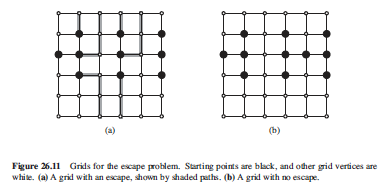
\includegraphics[width=\linewidth]{images/worksheet_5_1.png}
        \end{center}
    \end{enumerate}
\end{enumerate}

\end{document}